\documentclass[a4j,10pt]{jarticle}
\usepackage[dvipdfm,text={175mm,260mm},centering]{geometry}
\usepackage{newtxtext,newtxmath}
\usepackage[dvipdfmx]{graphicx}
\usepackage{listings,jvlisting}
\usepackage{color}
\usepackage{tabularx}
\usepackage{booktabs}
\usepackage{multirow}
\usepackage{comment}
\usepackage{tikz} 
\usetikzlibrary{arrows.meta}

% 担当教員名
\newcommand{\teacherName}{桝井 晃基}
% 提出者名
\newcommand{\studentName}{鶴見 俊介}
% 提出者所属
\newcommand{\studentAff}{基礎工学部 情報科学科3年 計算機科学コース}
% 提出者学籍番号
\newcommand{\studentID}{09B23057}
% 提出者電子メールアドレス
\newcommand{\studentEmail}{u299151f@ecs.osaka-u.ac.jp}
% 課題提出日
\newcommand{\submitted}{\today}
% 課題締め切り日
\newcommand{\deadline}{2025年12月12日}

\lstset{
    basicstyle = {\ttfamily},
    backgroundcolor  = {\color[gray]{.99}},
    breaklines = true,
    columns = [l]{fullflexible},
    commentstyle = {\smallitshape},
    frame = {tb},
    identifierstyle = {\small},
    keepspaces=true,
    keywordstyle = {\small\bfseries},
    lineskip = -0.5ex,
    ndkeywordstyle = {\small},
    numbers = left,
    numbersep = 1zw,
    numberstyle = {\scriptsize},
    stepnumber = 1,
    stringstyle = {\small\ttfamily},
    xleftmargin = 3zw,
    xrightmargin = 0zw
}
\renewcommand{\lstlistingname}{プログラム}

\begin{document}
\begin{titlepage}
\begin{center}
{\Huge\bfseries 情報科学演習D} \\
\vspace{1cm}
{\LARGE\bfseries 課題3}
\vspace{5cm}

{\large
\begin{tabular}{rcl}
担当教員 & : & \teacherName \\
提出者   & : & \studentName \\
所属/学年   & : & \studentAff\\
学籍番号 & : & \studentID \\
電子メール & : & \texttt{\studentEmail}\\
&& \\
提出日 & : & \submitted \\
締切日 & : & \deadline
\end{tabular}
}
\end{center}
\end{titlepage}

\setcounter{tocdepth}{2}
% \tableofcontents
\newpage

% コマンド一覧
\begin{comment}
    \lstinputlisting[caption=, firstline=1, firstnumber=1, lastline=, label=prog:]{codes/}
\end{comment}

\begin{comment}
\begin{figure}[htb]
    \centering
    \caption{}
    \includegraphics[]{}
    \label{}
\end{figure}
\end{comment}



% 以下本文

\section{システムの仕様}
本システムは，\verb|Pascal| 風言語プログラムの字句解析結果（\verb|ts| ファイル）に対して構文解析および意味解析を行い，結果を文字列で返す意味解析器である．
エントリポイントは \verb|enshud.s3.checker.Checker| クラスの\verb|run(String)| メソッドとする．

\verb|run| メソッドは，入力として \verb|ts| ファイル名\verb|inputFileName| を受け取り，次のいずれかの文字列を返す．

\begin{itemize}
  \item 入力ファイルが存在しない場合：\verb|"File not found"|
  \item 構文解析で最初に検出された構文誤りの行が \verb|n| のとき：
        \verb|"Syntax error: line n"|
  \item 構文的に正しい場合に，意味解析で最初に検出された意味誤りの行が \verb|n| のとき：
        \verb|"Semantic error: line n"|
  \item 構文・意味のいずれの解析でも誤りが検出されなかった場合：\verb|"OK"|
\end{itemize}

\section{課題達成の方針と設計}

\subsection{設計方針とクラス構成}

本課題の意味解析器は，構文解析で得られた \verb|AST| を入力として，
\verb|Visitor| パターンにより 1 回の走査で宣言チェックと型検査を行う方針とした．
\verb|Checker.run| はまず \verb|ts| ファイルを読み込み，構文解析器を用いて
\verb|Program| ノードを根とする \verb|AST| を生成する．
この段階で構文誤りが検出された場合には意味解析を行わず，
メッセージ \verb|"Syntax error: line n"| を返す．
構文的に正しければ \verb|Program| ノードを意味解析器 \verb|Semantic| に渡し，意味解析を開始する．

図\ref{fig:class} に，意味解析に関わる主要クラスの関係を示す．
\verb|Semantic| は \verb|AstVisitor| インタフェースを実装していて，
\verb|Program.accept(this)| を起点として各種 \verb|visit*| メソッドを通じて
\verb|AST| 全体を巡回する．
識別子情報は \verb|SymbolTable| が管理し，\verb|Symbol| には
\verb|name|，\verb|kind|，\verb|type|，\verb|paramTypes| などを保持させることで，
変数・仮引数・手続きの宣言と参照を一元的に扱えるようにした．
また，\verb|Type| クラスは組み込み型や配列型を表現し，各式ノードに対する
\verb|visit*| の戻り値として使用することで，代入文，条件式，演算子，手続き呼び出しなどの
型整合性検査を一貫して行う．

図\ref{fig:sequence} は，\verb|Checker| と \verb|Semantic|，\verb|SymbolTable| を中心とした
意味解析処理の流れをシーケンス図として表したものである．
\verb|Checker| が \verb|Semantic| を生成すると，
\verb|Semantic| は最初に \verb|SymbolTable.enterScope()| でグローバルスコープを作成し，
続いて \verb|Program.accept(this)| により \verb|AST| 走査を開始する．
各 \verb|visit*| メソッド内では，宣言ノードに対して識別子の登録と重複宣言の検査を行い，
式ノードに対しては \verb|Type| を計算して親ノードに返すことで，上位構造の型チェックに利用する．
いずれかの \verb|visit*| で意味的な誤りを検出した場合には \verb|CheckError| 例外を送出し，
\verb|Checker.run| がこれを捕捉して最初の 1 件のみを \verb|"Semantic error: line n"| として報告する．

\begin{figure}[htb]
  \centering
  % 左：クラス図
  \begin{minipage}{0.51\linewidth}
    \centering
    
\includegraphics[width=\linewidth]{images/checker/checker.pdf}
    \caption{意味解析に関わるクラス図}
    \label{fig:class}
  \end{minipage}
  \hfill
  % 右：シーケンス図
  \begin{minipage}{0.42\linewidth}
    \centering
    
\includegraphics[width=\linewidth]{images/sequence/sequence.pdf}
    \caption{意味解析処理のシーケンス図}
    \label{fig:sequence}
  \end{minipage}

\end{figure}




\subsection{スコープ管理とシンボル表の設計}

本実装では，プログラム本体および手続き宣言の入れ子構造に対応して，
図\ref{fig:scope-and-stack} (a) のような静的スコープ構造を前提とする．
各スコープは，その領域で有効な識別子（変数・仮引数・手続き名）と
対応する \verb|Symbol| 情報（\verb|name|，\verb|kind|，\verb|type| など）を保持する単位であり，
グローバルスコープの内部に手続き \verb|A| のスコープ，さらにその内部に手続き \verb|B| のスコープが
入れ子になる形で表現される．

\verb|SymbolTable| は，この静的スコープ構造を図\ref{fig:scope-and-stack} (b) のような
「スコープのスタック」として管理する．
\verb|Semantic| が \verb|AST| を走査する際に，
プログラム開始時および各手続きの本体に入る直前で \verb|enterScope()| を呼び出し，
対応するスコープフレームをスタックに \verb|push| する．
手続き本体の末尾やプログラム末尾では \verb|exitScope()| によりフレームを \verb|pop| し，
スコープから抜けた識別子は以降の名前解決の対象外となる．

宣言ノードに対しては，現在スコープに対して \verb|declare()| を呼び出し，
同一スコープ内に同名シンボルが存在する場合は重複宣言として \verb|CheckError| を送出する．
一方，変数・配列・手続き呼び出しなど参照側のノードでは \verb|lookup()| を用いて，
スタックトップから順に外側スコープへ探索することで静的スコープ規則に従った名前解決を実現し，
見つからなかった場合は未宣言識別子のエラーとして扱う．

\begin{figure}[htbp]
  \centering

  % ===== 左：入れ子スコープ =====
  \begin{minipage}{0.55\linewidth}
    \centering
    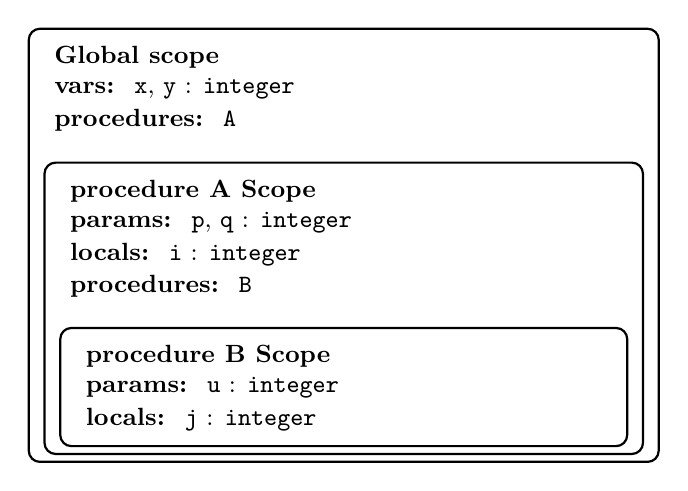
\begin{tikzpicture}[font=\small]

      % Global scope の枠
      \draw[rounded corners, thick] (-4,2.5) rectangle (4,-3.0);

      % Global scope のラベルと中身
      \node[anchor=north west] at (-3.8,2.4) {\textbf{Global scope}};
      \node[anchor=north west] at (-3.8,2.0)  {\textbf{vars:} \ \texttt{x}, \texttt{y} : \texttt{integer}};
      \node[anchor=north west] at (-3.8,1.6)  {\textbf{procedures:} \ \texttt{A}};

      % Procedure A のスコープ
      \draw[rounded corners, thick] (-3.8,0.8) rectangle (3.8,-2.9);
      \node[anchor=north west] at (-3.6,0.7) {\textbf{procedure A Scope}};
      \node[anchor=north west] at (-3.6,0.3) {\textbf{params:} \ \texttt{p}, \texttt{q} : \texttt{integer}};
      \node[anchor=north west] at (-3.6,-0.1) {\textbf{locals:} \ \texttt{i} : \texttt{integer}};
      \node[anchor=north west] at (-3.6,-0.5) {\textbf{procedures:} \ \texttt{B}};

      % Procedure B のスコープ
      \draw[rounded corners, thick] (-3.6,-1.3) rectangle (3.6,-2.8);
      \node[anchor=north west] at (-3.4,-1.4) {\textbf{procedure B Scope}};
      \node[anchor=north west] at (-3.4,-1.8) {\textbf{params:} \ \texttt{u} : \texttt{integer}};
      \node[anchor=north west] at (-3.4,-2.2) {\textbf{locals:} \ \texttt{j} : \texttt{integer}};

    \end{tikzpicture}

    {\footnotesize (a) 静的スコープの入れ子構造}
  \end{minipage}
  \hfill
  % ===== 右：シンボル表スタック =====
  \begin{minipage}{0.40\linewidth}
    \centering
    \begin{tikzpicture}[font=\small]

      % Global scope フレーム
      \draw[rounded corners, thick] (-2,0) rectangle (2,1);
      \node at (0,0.5) {\texttt{Global scope}};

      % procedure A のスコープ
      \draw[rounded corners, thick] (-2,1.4) rectangle (2,2.4);
      \node at (0,1.9) {\texttt{procedure A Scope}};

      % procedure B のスコープ（トップ）
      \draw[rounded corners, thick] (-2,2.8) rectangle (2,3.8);
      \node at (0,3.3) {\texttt{procedure B Scope}};

      % スタックの向きを示す矢印
      \draw[->,thick] (2.5,0.1) -- (2.5,3.9);
      \node[anchor=west] at (2.6,0.1) {\footnotesize \texttt{bottom}};
      \node[anchor=west] at (2.6,3.6) {\footnotesize \texttt{top}};

      % enterScope / exitScope の説明
      \node[anchor=west] at (-2.0,-0.6) {\footnotesize \texttt{enterScope()} / \texttt{exitScope()} で};
      \node[anchor=west] at (-2.0,-1.0) {\footnotesize スコープを push / pop する};

    \end{tikzpicture}

    {\footnotesize (b) 意味解析中のシンボル表スタック}
  \end{minipage}

  \caption{静的スコープ構造と意味解析時のシンボル表スタックの対応}
  \label{fig:scope-and-stack}
\end{figure}



\subsection{検出対象エラー}
\begin{table}[htbp]
  \centering
  \caption{検出対象エラーと主な検出箇所}
  \label{tab:errors}
  \begin{tabular}{p{0.40\linewidth}p{0.59\linewidth}}
    \toprule
    エラー種別 & 検出方針 \\ \midrule
    変数・仮引数・手続き名の重複宣言 &
      \verb|SymbolTable.declare| で同一スコープ内の重複を検査し，重複時に \verb|CheckError| を送出する． \\
    未宣言の変数・手続き名の参照 &
      各種 \verb|visit*| から \verb|SymbolTable.lookup| を呼び，未登録であればエラーとする． \\
    配列以外に対する添字アクセス／添字式が整数型でない &
      \verb|visitArrayAccess|，\verb|visitArrayRef| で参照先の \verb|Type| が配列型かどうかと，
      添字式の型が \verb|integer| かどうかを検査する． \\
    代入文の左辺が配列型／左右の型不一致 &
      \verb|visitAssign| で左辺の \verb|isArray| と左右の \verb|Type| を確認し，不適切な場合にエラーとする． \\
    \verb|if|／\verb|while| 条件式が \verb|boolean| 以外 &
      \verb|visitIfS|，\verb|visitWhileS| で条件式の型が \verb|boolean| でない場合にエラーとする． \\
    演算子と被演算子の型不整合 &
      \verb|visitBinary|，\verb|visitUnary| で演算子ごとの許容型をチェックし，違反時にエラーとする． \\
    手続き呼び出しの引数個数・型の不一致 &
      \verb|visitProcCall| で \verb|Symbol.paramTypes| と実引数列を比較し，個数・型のいずれかが
      不一致であればエラーとする． \\
    \bottomrule
  \end{tabular}
\end{table}
本システムでは，課題文で要求されている代表的な意味的誤りをすべて検出対象とした．
そのうえで，各エラー種別について「どの \verb|visit*|／\verb|SymbolTable| メソッドで検査するか」をあらかじめ整理し，
実装時に抜け漏れが生じないようにした．
表\ref{tab:errors}に，エラー種別と主な検出箇所の対応を示す．

\section{実装プログラム}
\subsection{Visitorパターンによる意味解析クラス}

本実装では，意味解析器 \verb|Semantic| を \verb|AST| 全体に適用するために，\verb|Visitor| パターンを用いた．
\verb|Semantic| のコンストラクタ（プログラム\ref{prog:semanic}）では，まずグローバルスコープを作成した上で，
\verb|Program| ノードに対して \verb|prog.accept(this)| を呼び出し，意味解析を開始する．

\lstinputlisting[caption=Semanticコンストラクタ, firstline=1, firstnumber=1, lastline=5, label=prog:semanic]{codes/visit.txt}

\verb|Program| クラス側の \verb|accept|（プログラム\ref{prog:accept}）は，渡された \verb|AstVisitor| に対して
\verb|visitProgram(this)| を呼ぶだけの薄いラッパであり，「どの \verb|visit*| を呼ぶか」をノード側が決定する．
\verb|Semantic| の \verb|visitProgram|（プログラム\ref{prog:visit}）では，\verb|block| と \verb|main| に対して
再び \verb|accept(this)| を呼び出し，下位のノードへ処理を委譲する．この再帰を通じて，\verb|AST| 全体が
\verb|1| 回走査される．

\lstinputlisting[caption=Programクラス, firstline=14, firstnumber=1, lastline=17, label=prog:accept]{codes/visit.txt}

\lstinputlisting[caption=visitProgramメソッド, firstline=7, firstnumber=1, lastline=12, label=prog:visit]{codes/visit.txt}

\verb|Program| ノード自身は型を持たないため \verb|visitProgram| の戻り値は \verb|null| としているが，
式ノードの \verb|visit*| は \verb|Type| を返し，文ノードの \verb|visit*| は \verb|null| を返す，という方針で統一している．
このように，「\verb|Checker| \textrightarrow{} \verb|Program.accept(this)| \textrightarrow{} 各 \verb|visit*| \textrightarrow{} 子ノードの \verb|accept(this)| \textrightarrow{} ...」という流れを取ることで，
\verb|AST| の走査手順は \verb|accept|／\verb|visit*| の呼び分けに集約され，意味解析の個々の処理（シンボル表操作や型検査）は各 \verb|visit*| メソッドの中に局所化されるようになっている．
また，新たな解析処理を追加する場合でも，既存の \verb|AST| クラスを変更せずに済むといった利点が得られる．

\subsection{スコープ付きシンボル表の実装}

識別子の宣言と参照を扱うために，\verb|Symbol|，\verb|Type|，\verb|SymbolTable| を用意した．
\verb|Type| は基底型（\verb|BasicType|）と配列フラグ・添字範囲をまとめた型情報，\verb|Symbol| は識別子名（\verb|name|），種別（\verb|kind|：変数／仮引数／手続き），型（\verb|type|），宣言位置（\verb|line|）などを保持する．
\verb|SymbolTable| は「\verb|Map<String,Symbol>| のスタック」として実装し，\verb|enterScope()|／\verb|exitScope()| でスコープ境界を \verb|push|／\verb|pop| することで，図\ref{fig:scope-and-stack} のような静的スコープ構造を表現している．

宣言時には現在スコープに対して \verb|declare(Symbol sym)| を呼び，同一スコープ内に同名シンボルがあれば \verb|CheckError| を送出する．
参照時には \verb|lookup(String name, int line)| によりスタックのトップから順に探索し，最初に見つかった \verb|Symbol| を返すことで，外側のスコープも含めた名前解決と未宣言識別子の検出を行う．

意味解析側では，各種 \verb|visit*| からこのシンボル表を直接呼び出す．
例えば変数宣言ノード \verb|VarDecl| に対する \verb|visitVarDecl|（プログラム\ref{prog:vardecl}）では，
まず \verb|resolveType| で宣言型を \verb|Type| に変換し，\verb|x, y, z: integer;| のような複数同時宣言に対して，各名前ごとに \verb|Symbol| を生成して \verb|symtab.declare| で登録する．
手続き宣言や仮引数宣言も同様に \verb|declare| で登録し，代入文や式ノード側では \verb|lookup| を通じて \verb|Symbol| を取得して型検査に利用する，という役割分担になっている．
\lstinputlisting[caption=\texttt{VarDecl}の意味解析, label=prog:vardecl]{codes/varDecl.txt}

\section{考察や工夫点}

本課題では，\verb|Parser| による \verb|AST| 構築を前提に，意味解析を \verb|Checker|・\verb|Semantic|・\verb|SymbolTable| の 3 クラスに分離した．
\verb|Checker| は入出力と例外処理のみを担当し，実際の走査と検査は \verb|Semantic|，識別子管理は \verb|SymbolTable| に委譲することで，
構文解析と意味解析の責務分離と，意味規則の追加・変更の局所化を図った．

スコープ管理については，図\ref{fig:scope-and-stack} のような静的スコープ構造を，そのまま \verb|SymbolTable| 内の
スコープスタックに写像する設計とした．\verb|enterScope()|／\verb|exitScope()| によりスコープの \verb|push|／\verb|pop| を行い，
\verb|declare()| は「現在スコープ内での重複宣言のみ」を検出する．一方 \verb|lookup()| はスタックのトップからボトムへ線形探索することで，
内側の宣言が外側を隠す静的スコープ規則を自然に実現している．これにより，入れ子の手続き宣言に対しても，単純なスタック操作で一貫した
名前解決が行えるようになった．

型検査では，配列型を含む全ての型情報を \verb|Type| に集約し，基底型 \verb|base|（\verb|integer|／\verb|char|／\verb|boolean|）と
配列フラグ \verb|isArray|，添字範囲 \verb|lower|，\verb|upper| を持たせた．特に，\verb|visitArrayAccess| で配列変数に対する添字アクセスの際に
要素型（\verb|elementType()|）を返す設計としたことで，\verb|visitAssign| では「\verb|a[i]| の型」と右辺式の型を単純に比較するだけで
型一致判定ができるようになっている．各 \verb|visit*| が返す \verb|Type| の意味を慎重に決めたことが，全体の実装を簡潔に保つうえで重要であった．

手続き呼び出しの検査では，\verb|ProcedureDecl| の仮引数グループ（例：\verb|(Y, M, D: integer)|）を展開し，
各名前ごとに同じ \verb|Type| を \verb|Symbol.paramTypes| に順序付きで登録するようにした．これにより，
\verb|visitProcCall| では \verb|Symbol.paramTypes| と実引数リストを 1 対 1 で対応付けて個数と型の両方を比較できる．
途中で仮引数グループ単位で型リストを保持してしまい，引数比較に失敗するバグも生じたが，
\verb|Param| の構造と \verb|Symbol| の保持形式を見直すことで整合した設計に修正できた．

\section{感想}

本課題を通じて，教科書で見ていた静的スコープやシンボル表，\verb|Visitor| パターンによる \verb|AST| 走査といった概念を，自分で実装して動かせるレベルまで具体化できたと感じた．
特に，\verb|Type| や \verb|Param| の設計では，最初に安易な表現を選ぶと，後段の型比較や引数チェックが急速に複雑化して破綻することを経験し，抽象データ構造の設計がコンパイラ実装の成否を大きく左右することを実感した．

また，構文解析で構築した \verb|AST| を意味解析のみにとどまらず，拡張版との共通基盤として使い回せる形で整理できたのは大きな収穫である．
一方で，今回は変数の初期化状態や配列添字の範囲といった実行時情報に依存する誤りは扱っておらず，データフロー解析などを導入することで，より高度な意味解析へ拡張できる余地も見えた．
今後は，今回の設計を土台として，より高機能な検査やコンパイラ全体の構築にも発展させていきたい．


\end{document}